\chapter{VẬT LÍ HẠT NHÂN}
\section{Cấu tạo hạt nhân}
\subsection{Tóm tắt lí thuyết}
\begin{tomtat}
	\subsubsection{Mô hình đơn giản của nguyên tử}
	\paragraph{Thí nghiệm tán xạ hạt $\alpha$}
	Năm 1911, Ernest Rutherford đã tiến hành thí nghiệm bắn chùm hạt $\alpha$ lên lá vàng mỏng.
	\begin{center}
		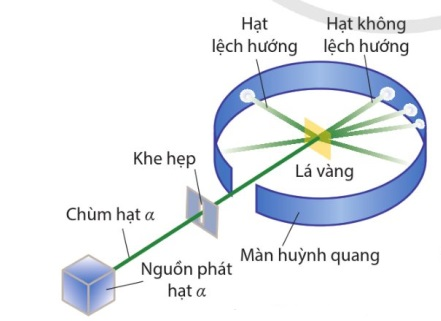
\includegraphics[width=0.4\linewidth]{figs/VN12-Y24-PH-SYL-025-1}
		\captionof{figure}{Sơ đồ thí nghiệm.}
	\end{center}
	\begin{enumerate}[label=\bfseries \alph*)]
		\item \textbf{Kết quả}\\
		Hầu hết các hạt $\alpha$ đi thẳng nhưng có một số ít hạt lệch so với hướng đi ban đầu (bị tán xạ) theo các góc khác nhau.
		\begin{center}
			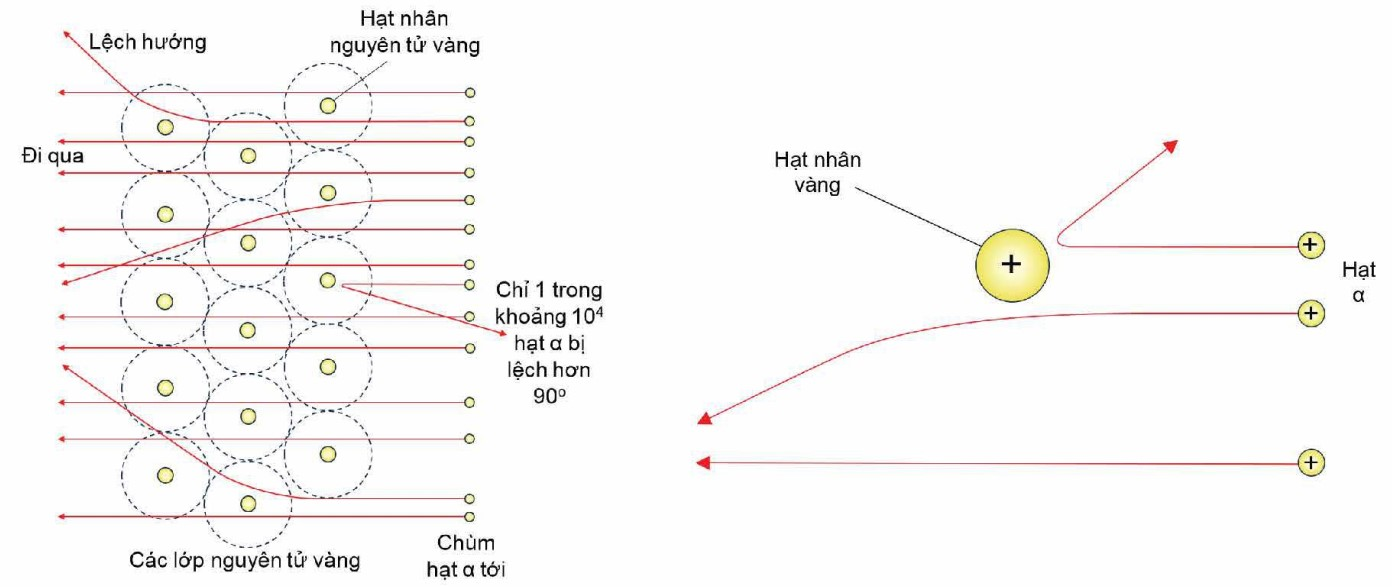
\includegraphics[width=0.9\linewidth]{figs/VN12-Y24-PH-SYL-025-2}
			\captionof{figure}{Minh hoạ kết quả thí nghiệm tán xạ hạt $\alpha$.}
		\end{center}
		\item \textbf{Nhận xét từ kết quả thí nghiệm}\\
		Phần lớn không gian bên trong nguyên tử là rỗng, toàn bộ điện tích dương trong nguyên tử chỉ tập trung tại một vùng có bán kính rất nhỏ nằm ở tâm của nguyên tử, là hạt nhân của nguyên tử.
	\end{enumerate}
	\paragraph{Mô hình đơn giản của nguyên tử}
	Từ thí nghiệm tán xạ hạt $\alpha$, Rutherford đã đưa ra mẫu hành tinh nguyên tử:
	\begin{center}
		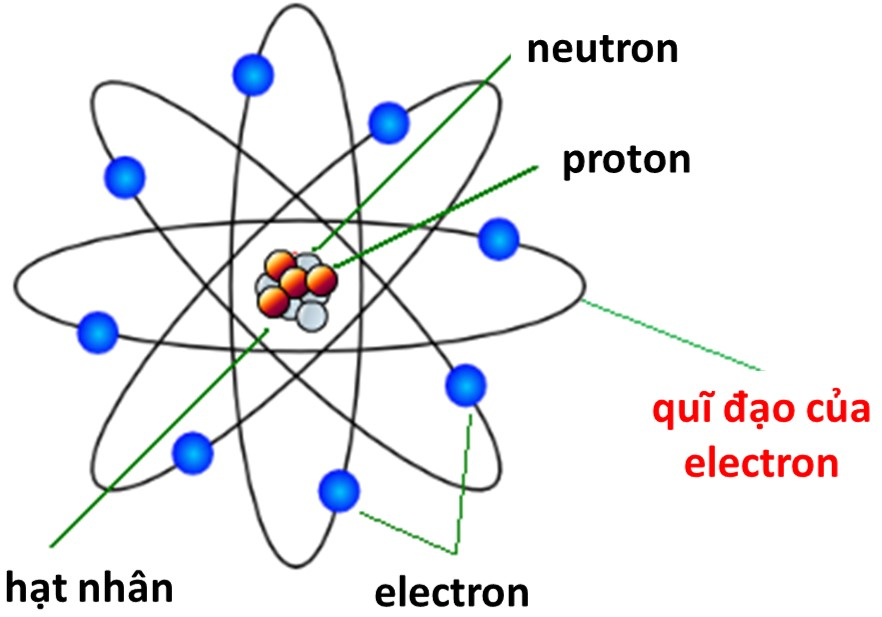
\includegraphics[width=0.3\linewidth]{figs/VN12-Y24-PH-SYL-025-3}
	\end{center}
	\begin{itemize}
		\item Nguyên tử có cấu trúc rỗng, với hạt nhân nguyên tử nằm ở tâm;
		\item Khối lượng nguyên tử tập trung chủ yếu ở hạt nhân;
		\item Điện tích hạt nhân có giá trị dương;
		\item Các electron chuyển động trên các quỹ đạo tròn xung quanh hạt nhân.
	\end{itemize}
	\subsubsection{Cấu tạo hạt nhân}
	\paragraph{Nucleon}
	Hạt nhân nguyên tử được cấu tạo bởi các nucleon. Có hai loại nucleon:
	\begin{itemize}
		\item Proton: kí hiệu $p$, mang điện tích nguyên tố dương $+e$, khối lượng $m_p\approx\SI{1.673E-27}{\kilogram}$.
		\item Neutron: kí hiệu $n$, không mang điện, khối lượng $m_n\approx\SI{1.675E-27}{\kilogram}$.
	\end{itemize}
	\begin{boxdl}
		Tổng số các nucleon trong hạt nhân được gọi là số khối:
		\begin{equation}
			A=Z+N
		\end{equation}
	\end{boxdl}
	trong đó
	\begin{itemize}
		\item $A$: số khối;
		\item $Z$: số proton = số thứ tự của nguyên tố đang xét trong bảng tuần hoàn các nguyên tố hoá học, được gọi là số hiệu nguyên tử;
		\item $N$: số neutron trong hạt nhân.
	\end{itemize}
	\paragraph{Kí hiệu hạt nhân}
	Hạt nhân của nguyên tử nguyên tố hoá học $X$ được kí hiệu là $^A_Z\ce{X}$.
	\paragraph{Đồng vị}
\begin{dn}
		Đồng vị là những nguyên tử mà hạt nhân chứa cùng số proton $Z$ nhưng có số neutron $N$ khác nhau.\\
	\textbf{\textit{Ví dụ:}} Carbon có 3 đồng vị chính là $^{12}_{\ 6}\ce{C}$, $^{13}_{\ 6}\ce{C}$ và  $^{14}_{\ 6}\ce{C}$. Trong đó, $^{12}_{\ 6}\ce{C}$ và $^{13}_{\ 6}\ce{C}$ là đồng vị bền, chiếm khoảng $\SI{99}{\percent}$ lượng carbon trong tự nhiên, $^{14}_{\ 6}\ce{C}$ là đồng vị phóng xạ.
\end{dn}
	\begin{luuy}
		Các đồng vị có cùng tính chất hoá học \textit{(do có cùng vị trí trong bảng phân loại tuần hoàn)} và có tính chất vật lí nói chung khác nhau.
	\end{luuy}
	\paragraph{Kích thước hạt nhân}
	\begin{boxdl}
		Hạt nhân được coi là hình cầu có bán kính
		\begin{equation}
			R=R_0A^{\frac{1}{3}}
		\end{equation}
		với $A$ là số khối hạt nhân và $R_0=\SI{1.2}{\femto\meter}=\SI{1.2E-15}{\meter}$.\\
		Thể tích của hạt nhân
		\begin{equation}
			V=\dfrac{4}{3}\pi R^3=\dfrac{4}{3}\pi R^3_0A.
		\end{equation}
	\end{boxdl}
\end{tomtat}
\subsection{Ví dụ minh hoạ}
\begin{dang}{Biểu diễn được kí hiệu hạt nhân của nguyên tử bằng số nucleon và số proton}
	\end{dang}
\begin{vd}
	Cho hai hạt nhân $^4_2\ce{He}$ và $^{31}_{15}\ce{P}$. Biết độ lớn điện tích nguyên tố là $e=\SI{1.6E-19}{\coulomb}$. Xác định số neutron và điện tích của mỗi hạt nhân.
	\loigiai{Hạt nhân $^4_2\ce{He}$ có $A=4$; $Z=2$ nên
		\begin{itemize}
			\item Số neutron là $N=A-Z=2$.
			\item Điện tích $q=+Ze=\SI{3.2E-19}{\coulomb}$.
		\end{itemize}	
		Hạt nhân $^{31}_{15}\ce{P}$ có $A=31$; $Z=15$ nên
		\begin{itemize}
			\item Số neutron là $N=A-Z=16$.
			\item Điện tích $q=+Ze=\SI{2.4E-18}{\coulomb}$.
	\end{itemize}	}
\end{vd}
% =============================================================
\begin{vd}
Nếu coi hạt nhân là một quả cầu thì hạt nhân thiếc (tin) $^{120}_{50}\ce{Sn}$ có bán kính và thể tích xấp xỉ bằng bao nhiêu?
\loigiai{
Bán kính hạt nhân:
$$R=1,2\cdot10^{-15}\cdot A^{\frac{1}{3}}\approx\SI{5.92E-15}{\meter}.$$
Thể tích của hạt nhân:
$$V=\dfrac{4}{3}\pi R^3\approx\SI{8.686E-43}{\meter^3}.$$	
}
\end{vd}
% ==============================================================
\begin{vd}
Coi khối lượng hạt nhân tính theo đơn vị u bằng số khối của nó và $\SI{1}{u}=\SI{1.66055E-27}{\kilogram}$. Tính khối lượng riêng của hạt nhân helium $^4_2\ce{He}$ và hạt nhân chì (lead) $^{206}_{82}\ce{Pb}$. 
\loigiai{
Khối lượng riêng của hạt nhân:
$$D=\dfrac{m}{\dfrac{4}{3}\pi R^3}=\dfrac{A\cdot u}{\dfrac{4}{3}\pi R^3_0 A}=\dfrac{u}{\dfrac{4}{3}\pi R^3_0}.$$
Như vậy, nếu xem khối lượng hạt nhân tính theo đơn vị u bằng số khối của nó thì các hạt nhân có khối lượng riêng như nhau:
$$D_{\ce{He}}=D_{\ce{Pb}}=\dfrac{\left(\SI{1.66055E-27}{\kilogram}\right)}{\dfrac{4}{3}\pi\cdot\left(\SI{1.2E-15}{\meter}\right)^3}\approx\SI{2.29E17}{\kilogram/\meter^3}.$$	
}
\end{vd}
% =========================================================
\begin{vd}
	Một nguyên tử X có tổng số hạt là 137, trong đó số hạt mang điện nhiều hơn số hạt trung hoà về điện là 31. Xác định số proton; số neutron và số nucleon của hạt nhân nguyên tử X.
	\loigiai{
Các hạt mang điện trong nguyên tử là electron và proton. Trong đó, số proton = số electron $=Z$.\\
Theo đề bài, ta có:
\begin{align*}
	\begin{cases}
		2Z+N=137\\
		2Z-N=31
	\end{cases}
	\Rightarrow \begin{cases}
		Z=42\\
		N=53
	\end{cases}
\end{align*}	
Số nucleon trong hạt nhân X là:
$$A=Z+N=95.$$	
	}
\end{vd}
\begin{dang}{Xác định tỉ lệ đồng vị của một nguyên tố}
	\end{dang}
\begin{vd}
Bạc (silver) có hai đồng vị ổn định: đồng vị 107 $\ce{Ag}$ có khối lượng nguyên tử là $\SI{106.905095}{u}$ chiếm $\SI{51.83}{\percent}$, còn lại là đồng vị 109 $\ce{Ag}$ có khối lượng nguyên tử là $\SI{108.904754}{u}$. Tính khối lượng nguyên tử trung bình của bạc.
\loigiai{Khối lượng trung bình của nguyên tử bạc:
	$$\overline{m}=\dfrac{\SI{106.905095}{u}\cdot51,83+\SI{108.904754}{u}\cdot48,17}{100}\approx\SI{107.868331}{u}.$$	}
\end{vd}
\subsection{Bài tập}
\subsubsection{Trắc nghiệm nhiều phương án lựa chọn}
\setcounter{ex}{0}
\Opensolutionfile{ans}[ans/VN12-Y24-PH-SYL-025P-TN]
% ===================================================================
\begin{ex}
	Hạt nhân nguyên tử gồm
	\choice
	{electron và proton}
	{neutron và electron}
	{\True neutron và proton}
	{electron và pozitron}
	\loigiai{}
\end{ex}


% ===================================================================
\begin{ex}
	Các nguyên tử được gọi là đồng vị khi hạt nhân của chúng có cùng
	\choice
	{khối lượng}
	{số neutron}
	{số nucleon}
	{\True số proton}
	\loigiai{}
\end{ex}
% ===================================================================
\begin{ex}
	Một hạt nhân nguyên tử có kí hiệu $\ce{_9^{19}X}$, kết luận nào dưới đây là \textbf{đúng}?
	\choice
	{X là nguyên tố có số thứ tự 19 trong bảng hệ thống tuần hoàn}
	{\True Hạt nhân này có 19 nucleon}
	{Hạt nhân này có 9 proton và 19 neutron}
	{Hạt nhân này có 10 proton và 9 electron}
	\loigiai{}
\end{ex}
% ===================================================================
\begin{ex}
	Hạt nhân $\ce{_6^{14}C}$ và hạt nhân $\ce{_7^{14}N}$ có cùng
	\choice
	{điện tích}
	{\True số nucleon}
	{số proton}
	{số neutron}
	\loigiai{}
\end{ex}
% ===================================================================
\begin{ex}
	Số hạt nucleon mang điện tích trong hạt nhân bạc $\ce{_{47}^{107}Ag}$ là
	\choice
	{\True 47}
	{60}
	{107}
	{154}
	\loigiai{}
\end{ex}

% ===================================================================
\begin{ex}
	Cặp nguyên tử của các hạt nhận nào sau đây không được gọi là đồng vị?
	\choice
	{$\ce{Cl}_{17}^{35} $, $\ce{Cl}_{17}^{37}$}
	{$\ce{H}_{1}^{1} $, $\ce{D}_{1}^{2}$}
	{$\ce{Cu}_{29}^{63} $, $\ce{Cu}_{29}^{65}$}
	{\True $\ce{H}_{1}^{3}$, $\ce{He}_{2}^{3}$}
	\loigiai{}
\end{ex}
% ===================================================================
\begin{ex}
	Hạt nhân nào sau đây có 136 neutron?
	\choice
	{$\ce{_{11}^{23}Na}$}
	{$\ce{_{92}^{238}U}$}
	{\True$\ce{_{86}^{222}Ra}$}
	{$\ce{_{84}^{209}Po}$}
	\loigiai{}
\end{ex}% ===================================================================
\begin{ex}
	Hạt nhân ${_{15}^{31}P}$ có
	\choice
	{31 proton và 15 neutron}
	{16 proton và 15 neutron}
	{\True15 proton và 16 neutron}
	{31 neutron và 15 proton}
	\loigiai{}
\end{ex}
% ===================================================================
\begin{ex}
	Hạt nhân nguyên tử $\ce{_{19}^{41}K}$ gồm
	\choice
	{19 proton và 41 neutron}
	{\True 19 proton và 22 neutron}
	{41 proton và 19 neutron}
	{22 proton và 19 neutron}
	\loigiai{}
\end{ex}
% ===================================================================
\begin{ex}
	Có 22 neutron trong đồng vị $\ce{^{42}Ca}$. Số proton trong đồng vị $\ce{^{40}Ca}$ là
	\choice
	{28}
	{26}
	{24}
	{\True 20}
	\loigiai{}
\end{ex}

% ===================================================================
\begin{ex}
	Sử dụng công thức về bán kính hạt nhân, hãy cho biết bán kính hạt nhân $\ce{_{82}^{207}Pb}$ lớn hơn bán kính hạt nhân $\ce{_{13}^{27}Al}$ bao nhiêu lần?
	\choice
	{Hơn 2,5 lần}
	{Hơn 2 lần}
	{\True Gần 2 lần}
	{1,5 lần}
	\loigiai{
		$$\dfrac{r_{\ce{Pb207}}}{r_{\ce{Al27}}}=\dfrac{A^{1/3}_{\ce{Pb207}}}{A^{1/3}_{\ce{Al27}}}=\dfrac{207^{1/3}}{27^{1/3}}\approx2.$$
	}
\end{ex}
% ===================================================================
\begin{ex}
	Phát biểu nào sau đây \textbf{sai}?	
	\choice
	{\True Đồng vị bền chỉ có nguồn gốc tự nhiên, đồng vị không bền chỉ có nguồn gốc nhân tạo}
	{Các nguyên tử mà hạt nhân có cùng số proton nhưng có số neutron khác nhau gọi là đồng vị}
	{Các đồng vị của cùng một nguyên tố có số neutron khác nhau nhưng tính chất hoá học giống nhau}
	{Các đồng vị của cùng một nguyên tố có cùng vị trí trong bảng hệ thống tuần hoàn}
	\loigiai{}
\end{ex}

% ===================================================================
\begin{ex}
	Trong các nhận định sau đây về kết quả thí nghiệm tán xạ của hạt alpha lên lá vàng mỏng, có bao nhiêu nhận định \textbf{đúng}?	
	\begin{enumerate}[label=(\arabic*)]
		\item Phần lớn các hạt alpha xuyên thẳng qua lá vàng mỏng.
		\item Một tỉ lệ khá lớn các hạt alpha bị lệch khỏi hướng ban đầu với góc lệch lớn hơn $\SI{90}{\degree}$.
		\item Một tỉ lệ rất nhỏ các hạt alpha bị lệch khỏi hướng ban đầu với góc lệch lớn hơn $\SI{90}{\degree}$.
		\item  Một số ít hạt alpha bị lệch khỏi phương ban đầu với những góc lệch khác nhau.
	\end{enumerate}
	\choice
	{1}
	{2}
	{\True 3}
	{4}
	\loigiai{
		Các nhận định đúng là: 1, 3 và 4.	
	}
\end{ex}
% ===================================================================
\begin{ex}
	So với hạt nhân $\ce{_6^{12}C} $, hạt nhân $\ce{_{27}^{56}Co}$ có nhiều hơn
	\choice
	{44 neutron và 21 proton}
	{\True 23 neutron và 21 proton}
	{44 neutron và 23 proton}
	{23 neutron và 23 proton}
	\loigiai{}
\end{ex}
% ===================================================================
\begin{ex}
	Trong nguyên tử của đồng vị phóng xạ $\ce{_{90}^{210}Th}$ có
	\choice
	{90 electron, tổng số proton và electron bằng 210}
	{\True 90 proton, tổng số neutron và electron bằng 210}
	{90 neutron, tổng số neutron và electron bằng 210}
	{90 neutron, tổng số proton và electron bằng 210}
	\loigiai{
		Số electron ở lớp vỏ nguyên tử bằng số proton bên trong hạt nhân.	
	}
\end{ex}
% ===================================================================
\begin{ex}
	Biết số Avogadro là $N_{A} \approx\SI{6.02E23}{\mole^{-1}}$, khối lượng mol của uranium $\ce{_{92}^{238}U }$ là $\SI{238}{\gram/\mole}$. Số neutron trong 238 gam $\ce{_{92}^{238}U }$ là	
	\choice
	{\True $8,79\cdot10^{25}$ hạt}
	{$27,7\cdot10^{24}$ hạt}
	{ $4,07\cdot10^{24}$ hạt}
	{$7,07\cdot10^{25}$ hạt}
	\loigiai{
		Số neutron có trong 1 hạt nhân $\ce{^{238}_{92}U}$ là: $238-92=\SI{146}{\text{hạt}}$.\\
		Suy ra: $N_n=146\cdot\dfrac{m}{A}\cdot N_A=146\cdot\dfrac{238}{238}\cdot 6,022\cdot10^{23}\approx\SI{8.79E25}{\text{hạt}}.$
	}
\end{ex}
% ===================================================================
\begin{ex}
	Cho số Avogadro $N_A=\SI{6.02E-23}{\mole^{-1}}$. Số neutron có trong $\SI{3.5}{\gram}$ carbon $\ce{_6^{14}C}$ có giá trị bằng
	\choice
	{$3,01 \cdot 10^{23}$}
	{$6,02 \cdot 10^{23}$}
	{$9,03\cdot10^{23}$}
	{\True $12,04\cdot10^{23}$}
	\loigiai{
		Số neutron có trong $\SI{3.5}{\gram}$ carbon $\ce{^{14}_6C}$ là
		$$N=\dfrac{m}{A}\cdot N_A\cdot\left(A-N_p\right)=\dfrac{\left(\SI{3.5}{\gram}\right)}{\left(\SI{14}{\gram/\mole}\right)}\cdot\left(\SI{6.02E23}{\mole^{-1}}\right)\cdot\left(14-6\right)=\SI{12.04E23}{}.$$	
	}
\end{ex}


\Closesolutionfile{ans}
\subsubsection{Trắc nghiệm đúng/sai}
\setcounter{ex}{0}
\Opensolutionfile{ans}[ans/VN12-Y24-PH-SYL-025P-TF]
% ===================================================================
\begin{ex}
	Trong mỗi phát biểu sau, em hãy chọn đúng hoặc sai.
	\choiceTFt
	{Hạt nhân nguyên tử trung hoà về điện}
	{\True Một hệ quả của mẫu nguyên tử Rutherford là tính không bền của nguyên tử do electron mất năng lượng khi chuyển động có gia tốc}
	{Hạt nhân nguyên tử được cấu tạo từ proton, neutron và electron}
	{Điện tích dương trong nguyên tử phân bố đều, xen kẽ với các electron nên nguyên tử trung hoà về điện}
	{\True Có thể xem khối lượng hạt nhân xấp xỉ bằng khối lượng nguyên tử}
	{\True Nguyên tử của đồng vị $\ce{_{27}^{60}Co }$ có 27 proton, 33 neutron và 27 electron}
	{\True Khi nguyên tử trung hoà về điện, tổng số electron và neutron bằng số khối của hạt nhân nguyên tử}
	{\True Nguyên tử chỉ tồn tại trong các trạng thái có năng lượng xác định, gọi là các trạng thái dừng. Khi ở trạng thái dừng, nguyên tử không phát xạ}
	\loigiai{}
\end{ex}

% ===================================================================
\begin{ex}
	Hình bên minh họa cấu tạo của một hạt nhân X. Biết độ lớn điện tích của nguyên tố là $e$.
	\begin{center}
		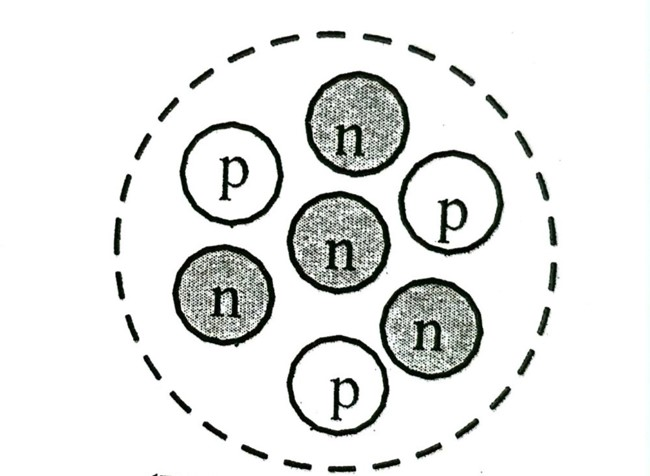
\includegraphics[width=0.3\linewidth]{figs/VN12-Y24-PH-SYL-027P-1}
	\end{center}
	\choiceTF[t]
	{Kí hiệu của hạt nhân là $\ce{^4_3X}$}
	{Điện tích của hạt nhân là $q=+7e$}
	{\True Nguyên tố X đứng vị trí thứ 3 trong bảng hệ thống tuần hoàn}
	{Số hạt mang điện của X nhiều hơn số hạt trung hòa về điện là 1}
	\loigiai{
		\begin{itemchoice}
			\itemch Sai. Nguyên tố này có 3 proton và 4 neutron. Kí hiệu là $\ce{^7_3X}$
			\itemch Sai. Điện tích là $q=+3e$.
			\itemch Đúng.
			\itemch Sai. Số hạt mang điện là 3 và số hạt trung hòa về điện là 4.
		\end{itemchoice}
	}
\end{ex}
% ===================================================================
\begin{ex}
	Hạt nhân X có cấu tạo gồm 7 hạt mang điện và 7 hạt trung hòa về điện.
	\choiceTF[t]
	{Số nucleon của X là 0}
	{Kí hiệu của X là $\ce{^7_7X}$}
	{\True Biết độ lớn điện tích nguyên tố là $e$. Điện tích của hạt X là $q=+7e$}
	{\True Bán kính của hạt nhân X là $R\approx\SI{2.9E-15}{\meter}$}
	\loigiai{
		\begin{itemchoice}
			\itemch Sai. Số nucleon của X là 14.
			\itemch Sai. Kí hiệu của X là $\ce{^{14}_7X}$.
			\itemch Đúng.
			\itemch Đúng.
		\end{itemchoice}
	}
\end{ex}
% ===================================================================
\begin{ex}
	Hình bên dưới là mô phỏng mẫu nguyên tử nguyên tố X theo mô hình của Rutherford.
	\begin{center}
		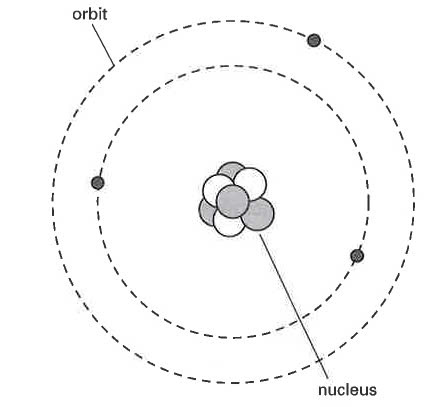
\includegraphics[width=0.25\linewidth]{figs/VN12-Y24-PH-SYL-026P-3}
	\end{center}
	Nhận định các phát biểu sau đây:
	
	\choiceTF[t]
	{\True Nguyên tử nguyên tố X có 3 electron}
	{Hạt nhân nguyên tử X có 10 nucleon}
	{Hạt nhân của nguyên tử X chứa 3 neutron}
	{\True Các electron ở gần hạt nhân chuyển động với tốc độ lớn hơn các electron ở lớp ngoài cùng}
	\loigiai{
		\begin{itemchoice}
			\itemch Đúng.
			\itemch Sai. Hạt nhân nguyên tử X có chứa 7 nucleon.
			\itemch Sai. Hạt nhân nguyên tử X chứa 4 neutron.
			\itemch Đúng. Các electron càng gần hạt nhân chuyển động với tốc độ càng lớn.
		\end{itemchoice}	
	}
\end{ex}
\Closesolutionfile{ans}
\subsubsection{Tự luận}
\setcounter{ex}{0}
\Opensolutionfile{ans}[ans/VN12-Y24-PH-SYL-025P-TL]
% ======================================================================
\begin{ex}
	Điền các số liệu còn thiếu vào bảng sau.
	\begin{center}
		\begin{tabular}{|l|M{4cm}|M{4cm}|M{4cm}|}
			\hline Kí hiệu tên nguyên tố & $\ce{O}$ & $\ce{K}$ & $\ce{Na}$ \\
			\hline Số proton & 8 & & 11 \\
			\hline Số neutron & & 20 & 12 \\
			\hline Số khối & 16 & 39 &\\
			\hline Kí hiệu hạt nhân & & & \\
			\hline
		\end{tabular}
	\end{center}
	\loigiai{
		\begin{center}
			\begin{tabular}{|l|M{4cm}|M{4cm}|M{4cm}|}
				\hline Kí hiệu tên nguyên tố & $\ce{O}$ & $\ce{K}$ & $\ce{Na}$ \\
				\hline Số proton & 8 &\textbf{19} & 11 \\
				\hline Số neutron & \textbf{8}& 20 & 12 \\
				\hline Số khối & 16 & 39 &\textbf{23} \\
				\hline Kí hiệu hạt nhân & $\ce{^{16}_8O}$ &$\ce{^{39}_{19}K}$ &$\ce{^{23}_{11}Na}$ \\
				\hline
			\end{tabular}
		\end{center}
	}
\end{ex}
% ======================================================================
\begin{ex}
	Tính bán kính của các hạt nhân nguyên tử $\ce{_2^4He}$, $\ce{_{92}^{235}U}$,  $\ce{_{26}^{56}Fe}$, $\ce{_{55}^{137}Cs}$ .	
	\loigiai{
		Áp dụng công thức $r=1,2\cdot10^{-15}\cdot A^{1/3}$, ta có:
		$r_{\ce{He}}=\SI{1.9}{\femto\meter}$; $r_{\ce{U}}=\SI{7.4}{\femto\meter}$; $r_{\ce{Fe}}=\SI{4.59}{\femto\meter}$; $r_{\ce{Cs}}=\SI{6.19}{\femto\meter}$.
		
	}
\end{ex}

% ======================================================================
\begin{ex}
	Giả sử hạt nhân nguyên tử có dạng hình cầu. Hỏi thể tích hạt nhân $\ce{_{26}^{56}Fe}$ gấp bao nhiêu lần thể tích hạt nhân $\ce{_1^3T}$?
	
	\loigiai{
		$$\dfrac{V_{\ce{Fe}}}{V_{\ce{T}}}=\dfrac{r^3_{\ce{Fe}}}{r^3_{\ce{T}}}=\dfrac{A_{\ce{Fe}}}{A_{\ce{T}}}=\dfrac{56}{3}\approx18,7.$$
	}
\end{ex}
% ======================================================================
\begin{ex}
	Nêu cấu tạo và viết kí hiệu hạt nhân của các nguyên tử trong các trường hợp sau:
	\begin{center}
		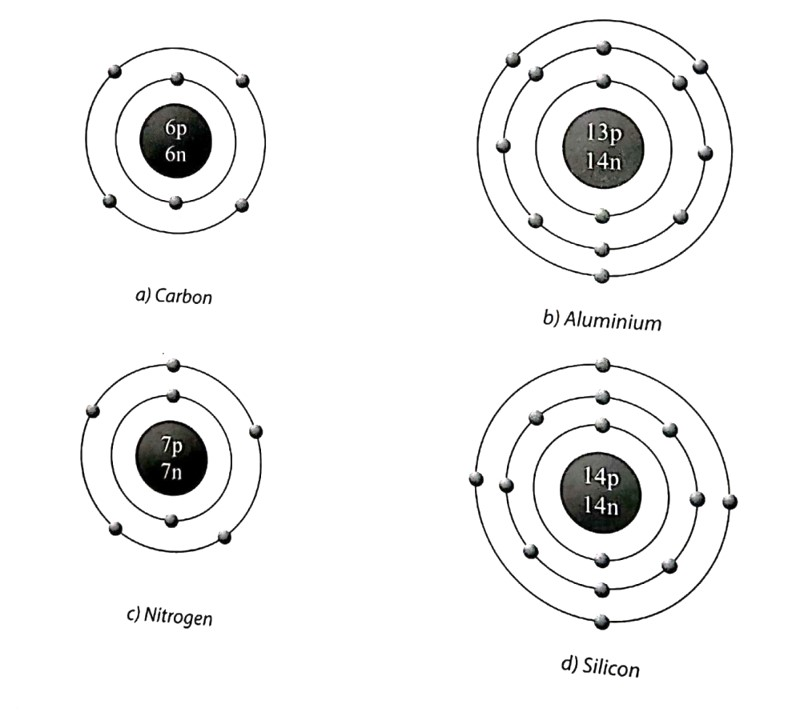
\includegraphics[width=0.5\linewidth]{figs/VN12-Y24-PH-SYL-026P-1}
	\end{center}
	\loigiai{
		\begin{enumerate}[label=\alph*)]
			\item Nguyên tử carbon: 6 proton, 6 neutron, 6 electron. Kí hiệu hạt nhân: $\ce{^{12}_6C}$.
			\item Nguyên tử aluminium: 13 proton, 14 neutron, 13 electron. Kí hiệu hạt nhân: $\ce{^{27}_{13}Al}$.
			\item Nguyên tử nitrogen: 7 proton, 7 neutron, 7 electron. Kí hiệu hạt nhân: $\ce{^{14}_7N}$.
			\item Nguyên tử silicon: 14 proton, 14 neutron, 14 electron. Kí hiệu hạt nhân: $\ce{^{28}_14Si}$.
		\end{enumerate}
	}
\end{ex}
% ===============================================================

\begin{ex}
	Ở giai đoạn cuối của quá trình tiến hoá sao, một ngôi sao có khối lượng gấp đôi khối lượng Mặt Trời sẽ suy sụp hấp dẫn ở nhân, tổng hợp proton và electron của nó lại để tạo thành sao neutron. Do đó, ngôi sao lúc này có thể được coi là một hạt nhân nguyên tử khổng lồ. Nếu một ngôi sao có khối lượng $2\times\SI{1.99E30}{\kilogram}$ suy sụp thành các neutron ($m_n=\SI{1.67E-27}{\kilogram}$)  thì bán kính sao neutron lúc này là bao nhiêu? Giả sử bán kính $r=r_0A^{\frac{1}{3}}$, với $r_0=\SI{1.2}{\femto\meter}$. Kết quả tính theo đơn vị kilomet và làm tròn đến 1 chữ số thập phân.
	\loigiai{
		Số neutron trong ngôi sao:
		$$A=\dfrac{m}{m_n}$$
		Bán kính sao:
		$$r=r_0A^{\frac{1}{3}}=r_0\left(\dfrac{m}{m_n}\right)^{\frac{1}{3}}=\left(\SI{1.2E-15}{\meter}\right)\cdot\left[\dfrac{2\times\SI{1.99E30}{\kilogram}}{\SI{1.67E-27}{\kilogram}}\right]^{\frac{1}{3}}
		\approx\SI{16028.9}{\meter}=\SI{16.03}{\kilo\meter}.$$}
\end{ex}

% ======================================================================
\begin{ex}
	Trong thí nghiệm tán xạ hạt $\alpha$ trên lá vàng mỏng, hạt $\alpha$ có khối lượng $\SI{6.64E-27}{\kilogram}$ phát ra từ nguồn với tốc độ $\SI{1.85E7}{\meter/\second}$ bay đến gần một hạt nhân vàng theo phương nối tâm hai hạt nhân như hình bên dưới.
	\begin{center}
		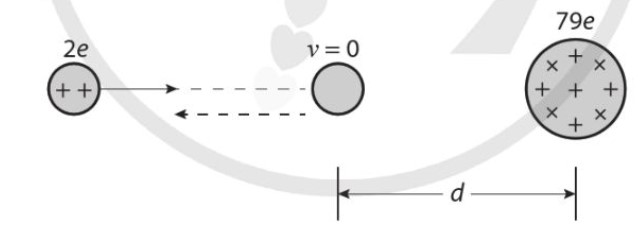
\includegraphics[width=0.4\linewidth]{figs/VN12-Y24-PH-SYL-026P-2}
	\end{center}
	Tính khoảng cách gần nhất $d$ giữa hạt $\alpha$ và hạt nhân vàng. Biết rằng ở khoảng cách đó, thế năng của hạt $\alpha$ trong điện trường gây bởi hạt nhân vàng được tính theo công thức $W_t=\dfrac{k Q_\alpha Q_{v}}{d}$, trong đó: $Q_\alpha$ và $Q_{v}$ lần lượt là điện tích của hạt $\alpha$ và hạt nhân vàng; $k=\SI{9E9}{\newton\meter^2/\coulomb^2}$. Cho biết $e=\SI{1.6E-19}{\coulomb}$.
	\loigiai{
		Khi được phóng ra từ nguồn ở rất xa hạt nhân vàng, hạt $\alpha$ có động năng:
		$$W_{\text{đ}}=\dfrac{1}{2}mv^2$$
		Khi dừng lại cách hạt nhân vàng một khoảng $d$, toàn bộ động năng ban đầu của hạt $\alpha$ đã chuyển hóa thành thế năng của nó trong điện trường gây bởi hạt nhân vàng:
		$$W_t=\dfrac{kQ_\alpha Q_v}{d}$$
		Ta có: $\dfrac{1}{2}mv^2=\dfrac{kQ_\alpha Q_v}{d}\Rightarrow d=\dfrac{2kQ_\alpha Q_v}{mv^2}=\SI{3.20E-14}{\meter}.$
	}
\end{ex}
\Closesolutionfile{ans}	
